% Chapter Template

% Main chapter title
%\chapter[toc version]{doc version}
\chapter{Background}

% Short version of the title for the header
%\chaptermark{version for header}

% Chapter Label
% For referencing this chapter elsewhere, use \ref{ChapterTemplate}
\label{Chapter2Background}

% Write text in here
% Use \subsection and \subsubsection to organize text

The main focus of this chapter is to provide the reader with the necessary background to understand the context and technical 
foundations of this project. The goal of the system is to automatically evaluate network topologies by validating 
configurations and executing tests across various devices within a virtual network.

Achieving this requires the integration of multiple technologies, as the system must support a wide range of features to 
deliver an automated solution. Key concerns include not only functionality but also scalability, since 
multiple students may interact with the platform concurrently, each requiring an isolated working environment.

To support these requirements, this chapter introduces core concepts and tools such as virtualization, web frameworks, 
administration automation and task processing. These components form the foundation upon which the system is built.

\section{Overview of Used Technologies}

  \subsection{Virtualization}
    Virtualization is the process of creating a virtual version of physical resources, such as routers, switches, or even
    entire computers. In the context of this project, it is used to create virtual machines to provide students with a 
    work environment consisting of a virtual network, itself comprised of various types of virtualized devices. This approach 
    enhances scalability and reduces costs, as it allows multiple virtual machines to be run on a single physical machine.

    Virtualization can be categorized into \textbf{emulation} and \textbf{simulation}. 

    \begin{itemize}
      \item \textbf{Emulation} is the process of creating a virtual version of a physical device in software, replicating its 
      behavior exactly—including any bugs and limitations. This is useful for various things like testing software on 
      different platforms, running legacy software on modern hardware and even running potentially harmful software in a safe 
      isolated environment.
      Emulation will be used wherever possible to provide students with a work environment that  matches the real world as much as 
      possible to best develop their network skills
      \item \textbf{Simulation} models the behaviour of a device, without replicating the underlying hardware or software.
      This results in a simpler less resource intensive model, though it may not fully capture the real device's behavior.
      Simulation will be used to simulate the behaviour of certain, simpler and generic, network devices and PCs.

    \end{itemize}


  \subsection{GNS3}
    \ac{gns3} is an open-source graphical network emulator software that allows the user to create complex network topologies 
    and interact with the various devices in it. It is widely used for educational purposes and is often used in preparation 
    for professional network certifications like the Cisco Certified Network Associate (CCNA).

    \ac{gns3} employs a simple drag and drop interface to allow users to add new devices, make links between them 
    and even add textual annotations. The software allows users to interact with the devices by way of a console or even a GUI
    if the device supports it. The software also allows users to export their topologies to be shared with others, which can
    be useful for teachers to provide students with a pre-configured topology to work on.

    Additionally, the software supports packet capturing which is essential for students to develop their debugging and 
    troubleshoting skills. Finally it can also be interacted with via a\ac{rest}\ac{api} which is of particular interest
    for this project.

  \subsection{Architecture}
    The software can be employed in a variety of ways due to its architecture \cite{GNS3Architecture} that separates the user 
    interfaces that it offers, namely the locally installed gns3-gui as well as the browser accessible gns3-web, from the 
    gns3-server that runs the emulations and the controller who orchestrates everything.

    \subsubsection{Controller}
      The controller is integrated in the gns3-server project and is responsible for communicating with all the other components 
      of the software. The controller is a singleton, meaning there should only be one instance of it running at any given time, 
      and it does not support concurrent requests. It is able to control multiple compute instances if so desired, each capable 
      of hosting one or more emulator instances, varying depending on their complexity. The controller also exposes the
      \ac{rest}\ac{api} allowing the ability to interact with the software programatically. All communication is done over
      \ac{http} in\ac{json} format and there is support for basic\ac{http} authentication as well as notifications via websockets.

    \subsubsection{Compute}
      The compute is also integrated in the gns3-server project and controls the various emulators required to run the nodes 
      in the topology.
      The list of currently supported emulators is:

      \begin{itemize}
          \item \textbf{Dynamips} - Used to emulate Cisco routers and basic switching.
          \item \textbf{\ac{iou}} - Used to emulate Cisco\ac{ios} devices.
          \item \textbf{\ac{qemu}} - Used to emulate a wide variety of devices.
          \item \textbf{\ac{vpcs}} - A basic program meant to simulate a basic PC.
          \item \textbf{VMware/VirtualBox} - Used to run virtual machines with nested virtualization support.
          \item \textbf{Docker} - Used to run docker containers.
        \end{itemize}

    \subsubsection{GUI}
      The GUI is composed of two separate but with mostly identical functionality, namely the gns3-gui and the gns3-web projects.
      The gns3-gui project is a desktop application that is used to to interact with a local or remote gns3-server instance. It 
      is written in Python and uses the Qt framework for the graphical interface. The gns3-web is a web interface that is 
      accessible via web browser and even though it is still in a beta stage, it has all the necessary features and stability to 
      be used as a substitute for the gns3-gui.

      \begin{figure}
          \centering
            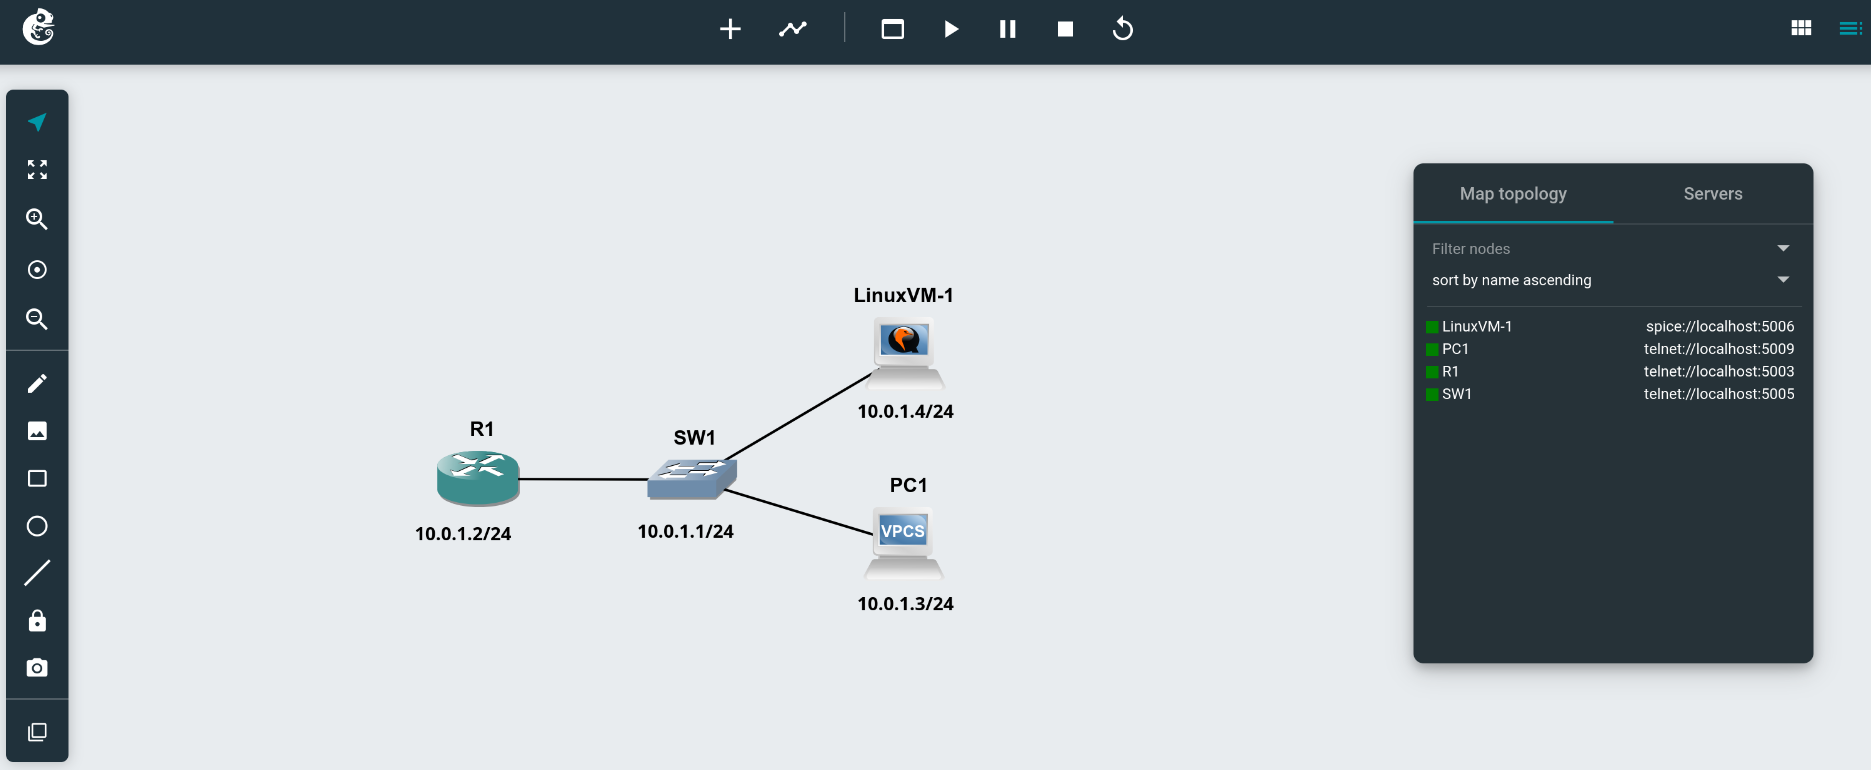
\includegraphics[width=.95\linewidth]
              {2Background/gns3-web.png}
          \caption{A simple network topology example in the GNS3 Web UI}
        \hfill
      \end{figure}


  \subsection{Proxmox VE} 
    \ac{pve} is an open-source platform designed for enterprise-level virtualization \cite{proxmox2025}. It is based on the Debian
    distribution of Linux and provides a web-based interface for managing virtual machines and containers. It is widely used
    in data centers and cloud environments, as it provides a scalable and reliable solution for virtualization.

    \ac{pve} bundles several core services that can be interacted with via shell commands, a web interface or by using
    the\ac{pve}\ac{rest}\ac{api}.
    These allow the user to interact with every service provided by\ac{pve}, in a plethora of ways, depending on the user's
    needs, skills and preferences. The web interface is the most user-friendly way to interact with the platform, as it
    provides a graphical interface for managing the cluster. The shell commands provide a more direct way to interact with the
    platform, allowing for more complex operations to be performed and opening the doors to scripting and automation. Finally,
    the\ac{pve}\ac{rest}\ac{api} allows for programmatic and remote interaction with the platform, enabling users to create custom
    applications that can interact with the platform.

    \subsubsection{Virtualization Technologies}
      \ac{pve} supports the the deployment and management of two distinct types of virtualization, namely,\ac{kvm} and\ac{lxc}.

      Users can interact with these virtualized environments via NoVNC, a simple web-based VNC client or\ac{spice} which is a more
      feature-rich protocol that provides better performance and more features than VNC.
      Both of these protocols support the use of a console-based interface, aswell as a full desktop graphical interface.

      \subsubsection{\ac{kvm}}
        \ac{kvm} is a virtualization solution provided by the Linux kernel. It leverages the hardware virtualization extensions 
        of modern processors to provide a full virtualization experience at near-native speeds. Supports a wide range of guest 
        operating systems making it a good choice for general purpose virtualization.

        In\ac{pve},\ac{kvm} is used as the core component for running virtual machines and is used alongside\ac{qemu}.

      \subsubsection{\ac{lxc}}
        Containerization is an operating system-level virtualization method that packages an application and its dependencies
        together into an isolated environment. Contrary to traditional\ac{vm} solutions, containers dont emulate hardware or require a 
        guest operating system relying instead on the host's kernel. This approach leads to a faster and more lightweight 
        virtualization solution, as they consume less memory and cpu resources.

        \ac{lxc} creates full system containers, capable of simulating a complete Linux distribution providing users with an 
        environment that behaves like a traditional\ac{vm} but with the speed and efficiency of a container.\ac{lxc} start 
        much faster than\ac{vm}s making them ideal for scenarios requiring rapid deployment and/or scaling.

        However, it's important to note that while containers offer a degree of isolation, they do not provide the same level of
        security as\ac{vm}s. This means that while they may not always be a suitable replacement for\ac{vm}s.

  \subsection{LDAP}

    \ac{ldap} is the foundation of user and device management in many institutions. Universities can rely on openLDAP and/or Microsoft's 
    Active Directory (its enterprise implementation) to handle student, faculty accounts and lab computer access, amongst other things.

    One of\ac{ldap}'s most popular implementations, OpenLDAP, had its initial release in 1998. The protocol's longevity stems from its 
    efficiency at handling large-scale authentication so much so that despite newer alternatives existing,\ac{ldap} remains entrenched 
    in academic environments due to its reliability and universal adoption. For our project,\ac{ldap} integration enables students 
    access to the system using their existing university credentials. 

    Two key factors make\ac{ldap} particularly valuable for this project: its standardized approach to user management 
    and pre-existing deployment in our target educational environments. Given the extensive use, it's desirable for our system to have the 
    capability to interact with LDAP in order to correctly authenticate users.

\section{Virtualized Lab Environments}
  The combined use of\ac{pve} as a virtualization platform and\ac{gns3} for network emulation presents a cost-effective solution for 
  scalable networking education. This approach offers significant benefits over physical lab infrastructures:

  \begin{itemize}
    \item \textbf{Resource Efficiency}: Single physical host can support multiple concurrent student environments
    \item \textbf{Operational Characteristics}:
    \begin{itemize}
        \item Accelerated environment provisioning through templates
        \item State preservation via\ac{pve}'s snapshot/restore functionality
        \item Support for diverse network operating systems through virtualization technologies
    \end{itemize}
  \end{itemize}

\section{Python Web Frameworks for API-Based Systems}

  \subsection{Python}
    Python is a high-level, interpreted programming language renowned for its readability and versatility. It supports 
    multiple programming paradigms, including procedural, object-oriented, and functional programming, making it suitable 
    for a wide array of applications.
    In the context of this project, Python serves as the primary programming language as its extensive standard library 
    and supportive community contribute to efficient development and maintenance of the project's codebase.

  \subsection{WSGI}
    The\ac{wsgi} is a pivotal standard for Python web application deployment, defining a consistent interface between web 
    servers and Python web applications/frameworks.

    Prior to\ac{wsgi}'s introduction\cite{pep333}, Python web frameworks were typically written against various server-specific APIs such as 
    CGI, FastCGI, or mod\_python. This diversity led to compatibility issues, limiting developers' choices of web servers and 
    frameworks, as not all frameworks supported all web servers and vice-versa. To address this fragmentation,\ac{wsgi} was 
    created as a standardized interface, promoting portability and flexibility in deploying Python web applications. 

    \ac{wsgi} serves as a bridge, enabling web servers to communicate with Python applications. It specifies a simple and universal 
    interface for web servers to forward requests to Python applications and for those applications to return responses. 
    This standardization allows developers to choose from a variety of web servers and Python frameworks without compatibility 
    concerns.

    Introduced in 2003 as PEP 333,\ac{wsgi} was later updated to PEP 3333 in 2010 to accommodate Python 3. These specifications 
    outline how web servers and Python applications should interact, ensuring a consistent and reliable deployment environment 
    across different platforms.

    The\ac{wsgi} standard consists of two main components:
    \begin{itemize}
      \item \textbf{Server/Gateway Side} - Responsible for receiving\ac{http} requests from clients and passing them to the 
      Python application. Then receives the response from the application and forwards it to the client. 
      \item \textbf{Application} - The Python application that processes requests and returns responses.
    \end{itemize}

    Additionally\ac{wsgi} has support for middleware components.\ac{wsgi} middleware is a Python callable that wraps another
    \ac{wsgi} application to observe or modify its behavior. Middleware can perform various functions, including request 
    preprocessing, response postprocessing, session management, and security checks. This modularity allows developers to 
    add functionality to their applications in a reusable and maintainable manner.

    The separation defined by\ac{wsgi} allows for flexibility and scalability in deploying Python web applications.

    Python\ac{wsgi} applications often use built-in servers, during development, provided by frameworks like Flask. 
    However, these servers typically aren't fully featured and aren't suitable for production environments. In production, WSGI 
    servers act as intermediaries between web servers (e.g., NGINX or Apache) and Python applications, handling incoming requests 
    and serving responses efficiently.

    \subsubsection{Flask}
      Flask is a web application micro framework written in Python, adhering to the\ac{wsgi} standard, designed to 
      facilitate the development of web applications by providing essential tools and features. Classified as a microframework, 
      Flask does not require particular tools or libraries, instead choosing to focus on simplicity and extensibility\cite{flask2025}.

      An example of how easy it is to develop a basic web application with flask is provided in the following small 
      piece of code.

      \begin{algorithm}
        \caption{Flask Hello World}\label{flask-hello-world}
        \begin{algorithmic}[1]
          \State \textbf{from} flask \textbf{import} Flask
          \State \textbf{app} = Flask(\_\_name\_\_)
          \State
          \State \textbf{@app.route('/')}
          \State \textbf{def} hello\_world():
          \State \hspace{1em} \textbf{return} 'Hello, World!'
          \State
          \State \textbf{if} \_\_name\_\_ == '\_\_main\_\_':
          \State \hspace{1em} app.run()
        \end{algorithmic}
      \end{algorithm}

  \subsection{ASGI}

    \ac{asgi} is an interface specification for Python web servers and applications. It is considered a spiritual successor to
    \ac{wsgi}, designed to provide a standard interface for asynchronous communication.\ac{asgi} was developed to address the 
    limitations of \ac{wsgi}, which was primarily designed for synchronous applications. Unlike\ac{wsgi},\ac{asgi} supports 
    handling multiple requests concurrently, making it suitable for modern web applications that require real-time features such 
    as WebSockets, long-lived connections, background tasks or the use of Python's async features.
    
    As development progressed, asynchronous task handling became a more central requirement, initially addressed by integrating 
    task queues. However, due to resource overhead and deployment complexity, they were phased out. This shift prompted an evaluation 
    of frameworks that offered native support for asynchronous operations.
    
    \subsubsection{FastAPI}
      
      FastAPI is a modern, high-performance web framework adopting the\ac{asgi} standard. It leverages open standards, such as 
      \ac{oas}, for defining path operations, parameters, and more, which in turn is based on the\ac{json} schema.
      FastAPI relies entirely on Python type declarations, making it more intuitive and lowering the barrier to entry to new 
      developers. This approach also simplifies the understanding and maintenance of the codebase.
      
      Built on top of Starlette, a lightweight\ac{asgi} framework, and Pydantic, a data validation library. FastAPI combines the 
      strengths of both to provide a powerful and flexible framework for building APIs with automatic data validation, 
      serialization and documentation generation, all of which significantly enhance developer productivity.
      
      Another key feature of FastAPI, being\ac{asgi}-compliant, is its built-in support for asynchronous programming, allowing 
      developers to write non-blocking code using Python's \textit{async}/\textit{await} keywords. This is particularly useful 
      for I/O-bound operations, such as database queries or network requests, as it allows the application to handle multiple 
      requests concurrently without blocking the application which is essential in projects such as this one where multiple 
      concurrent\ac{http} calls are made to interact with multiple devices and services concurrently, such as\ac{gns3} and\ac{pve}.
      
      Another powerful feature of FastAPI is its dependency injection system, that is very easy to use as it is automatically
      handled by the framework itselft. This allows for a clean and modular codebase, as dependencies can be easily injected into
      the various components of the application. This is especially useful in larger applications, where managing dependencies
      can become complex and cumbersome.
      
      A change from Flask to FastAPI laid the groundwork for more efficient handling of I/O-bound operations—such as network interactions 
      with\ac{pve} or\ac{gns3}, which will be of importance in future iterations of the project while also streamlining development thanks 
      to FastAPI's built-in request parsing, background task support, and integrated dependency injection system.

\section{Long running task processing approaches}

  \subsection{The need for asynchronous processing in API-heavy applications.}
    Modern\ac{api}-driven applications benefit tremendously from asynchronous programming paradigms to handle concurrent operations 
    efficiently. Traditional synchronous execution models, where each request blocks thread execution until completion, prove 
    inadequate for systems requiring high throughput and responsiveness. This limitation becomes particularly apparent in projects 
    like ours, which relies heavily on\ac{http} calls to various devices and services.

    The asynchronous model, implemented through Python's \texttt{async}/\texttt{await} syntax, offers several critical advantages:

    \begin{itemize}
        \item \textbf{Improved Resource Utilization}: A single thread can manage multiple concurrent I/O operations by yielding control during waiting periods
        \item \textbf{Enhanced Scalability}: Systems can handle higher concurrent user counts with the same hardware resources
        \item \textbf{Responsive Performance}: The application remains reactive even during long-running operations
    \end{itemize}

    Although Python has native asynchronous capabilities, libraries must be written with these in mind, meaning some may have limited 
    or even no support for these capabilities.
    
  \subsection{Asyncio}

    Asyncio is Python's built-in library for writing concurrent asynchronous code. It serves as the foundation for asynchronous operations 
    in many Python frameworks, enabling high-performance networking, web servers, database connections, distributed task queues, etc.. 

    Asynchronous I/O can be useful in cases of time-consuming operations, as while awaiting the finish of said tasks, it relinquishes control 
    so that other code can run in the meantime. This approach is particularly well-suited for I/O-bound operations—such as network 
    communication, file access, or database queries—where tasks would otherwise spend a significant amount of time waiting for external operations that 
    are outside of our control to complete. Rather than blocking the entire application during such waits, Asyncio allows other tasks to 
    execute in the meantime, leading to more efficient resource utilization and improved throughput.

    Overall, Asyncio provides the concurrency model that underpins efficient I/O performance. By embracing this model, 
    the project benefits from improved responsiveness, lower latency, and better scalability—especially under workloads that 
    involve heavy interaction with external services.

    Frameworks that leverage these capabilities natively, provide the foundation for building responsive, scalable\ac{api} 
    services.
    
  \subsection{Celery}
    Celery is an open source distributed task queue focused on real-time processing but also offers support for task scheduling.
    It is implemented in Python, but the underlying protocol can be implemented in any language. Celery requires a message broker 
    to function, such as Redis or RabbitMQ, which are responsible for queuing and distributing tasks from producers (clients) to 
    consumers (workers).

    When integrating Celery into their projects developers must mark functions they want to be processed as tasks with Celery provided 
    decorators (e.g. \texttt{@app.task}) which allows workers to then execute them asynchronously. The system shines in projects requiring 
    heavy computational or scheduled jobs, but brings with it non-negligible operational, developmental and resouce overhead, doubly so if 
    the project didn't already include the use of message brokers.

\section{System administration automation tools}

  Modern system administration increasingly relies on automation tools to manage complex infrastructure while maintaining reliability and 
  reproducibility. In our context, configuration management systems serve as the foundational layer for ensuring well-configured device states 
  across network environments.

  \subsection{Nornir}
  
    Nornir is an open-source automation framework written in Python, designed to provide a flexible and efficient 
    approach to network automation tasks\cite{nornir2025}. Unlike other automation tools that utilize customized 
    pseudo-languages, Nornir leverages pure Python code, offering developers the full power and versatility of the Python 
    ecosystem.

    Nornir supports multi-threaded task execution, allowing operations to run parallel across multiple devices.
    This capability enhances efficiency and reduces the time required enabling easy scaling to a large number of devices.

    The framework provides a robust inventory management system, enabling the organization of devices into groups and the 
    assignment of specific tasks to these groups. This structure facilitates targeted automation and simplifies complex 
    network operations.

    Finally, thanks to Nornir's architecture, it is highly extensible through its plugin system, allowing users to create 
    custom plugins for inventory management, task execution, and result processing. This modularity ensures that Nornir can 
    adapt to a wide range of network automation scenarios.

    Nornir makes it easy to write reusable tasks for configuration management and state validation which makes it 
    highly desirable in the context of this project. Its ability to handle concurrent operations will also ensure it can scale 
    alongside the rest of the project.

  \subsection{Ansible}

    Ansible is a widely adopted open-source automation platform that simplifies configuration management, application deployment, 
    and task automation through a declarative YAML-based approach. Unlike imperative scripting solutions, Ansible employs playbooks 
    to define system states, making automation accessible to both developers and operations teams while maintaining robust capabilities 
    for complex workflows.

    The platform operates on an agentless architecture, utilizing\ac{ssh} for connectivity, which eliminates the need for persistent software 
    on managed nodes. This design choice significantly reduces deployment overhead while maintaining secure communication through standard 
    protocols. Ansible's push-based execution model allows for immediate task execution across entire device inventories without requiring 
    pre-installed clients.

    Ansible remains a valuable tool in task automation and orchestration but, as was already discussed in\cite{santos2024} there are several 
    barriers to the adoption of Ansible in this project, mainly the difficulties encountered by utilizing the Telnet protocol for 
    communications with network devices that dont support the\ac{ssh} protocol .